\section{总体分析}
\subsection{数据特征分析}

\subsubsection{空间与地形}

16 个任务节点（1 个调度中心 O01 与 15 个服务区）的坐标为 WGS84 经纬度，节点地面海拔介于 127.7$\sim$444.5\,m，需保护人口合计 3422 人。由于经纬度直接计算欧氏距离会产生显著误差，本文统一先投影到米制平面坐标系再计算水平距离。区域 30\,m DEM 覆盖经度 $109.03^\circ\sim109.45^\circ$、纬度 $22.86^\circ\sim23.22^\circ$，高程范围 41.69$\sim$1132.86\,m。需要特别说明的是，附件 DEM 为\textbf{数字表面模型（DSM，含植被与建筑）}，本文按原样使用、不做“去建筑”处理，因此净空与遮挡判定结果\textbf{偏保守}，对安全性有利。地形对空中视距链路的影响已有较多实测研究，山地场景下的空-地信道建模可参考文献~\cite{cui2019mountainchannel}。

\begin{figure}[htbp]
	\centering
	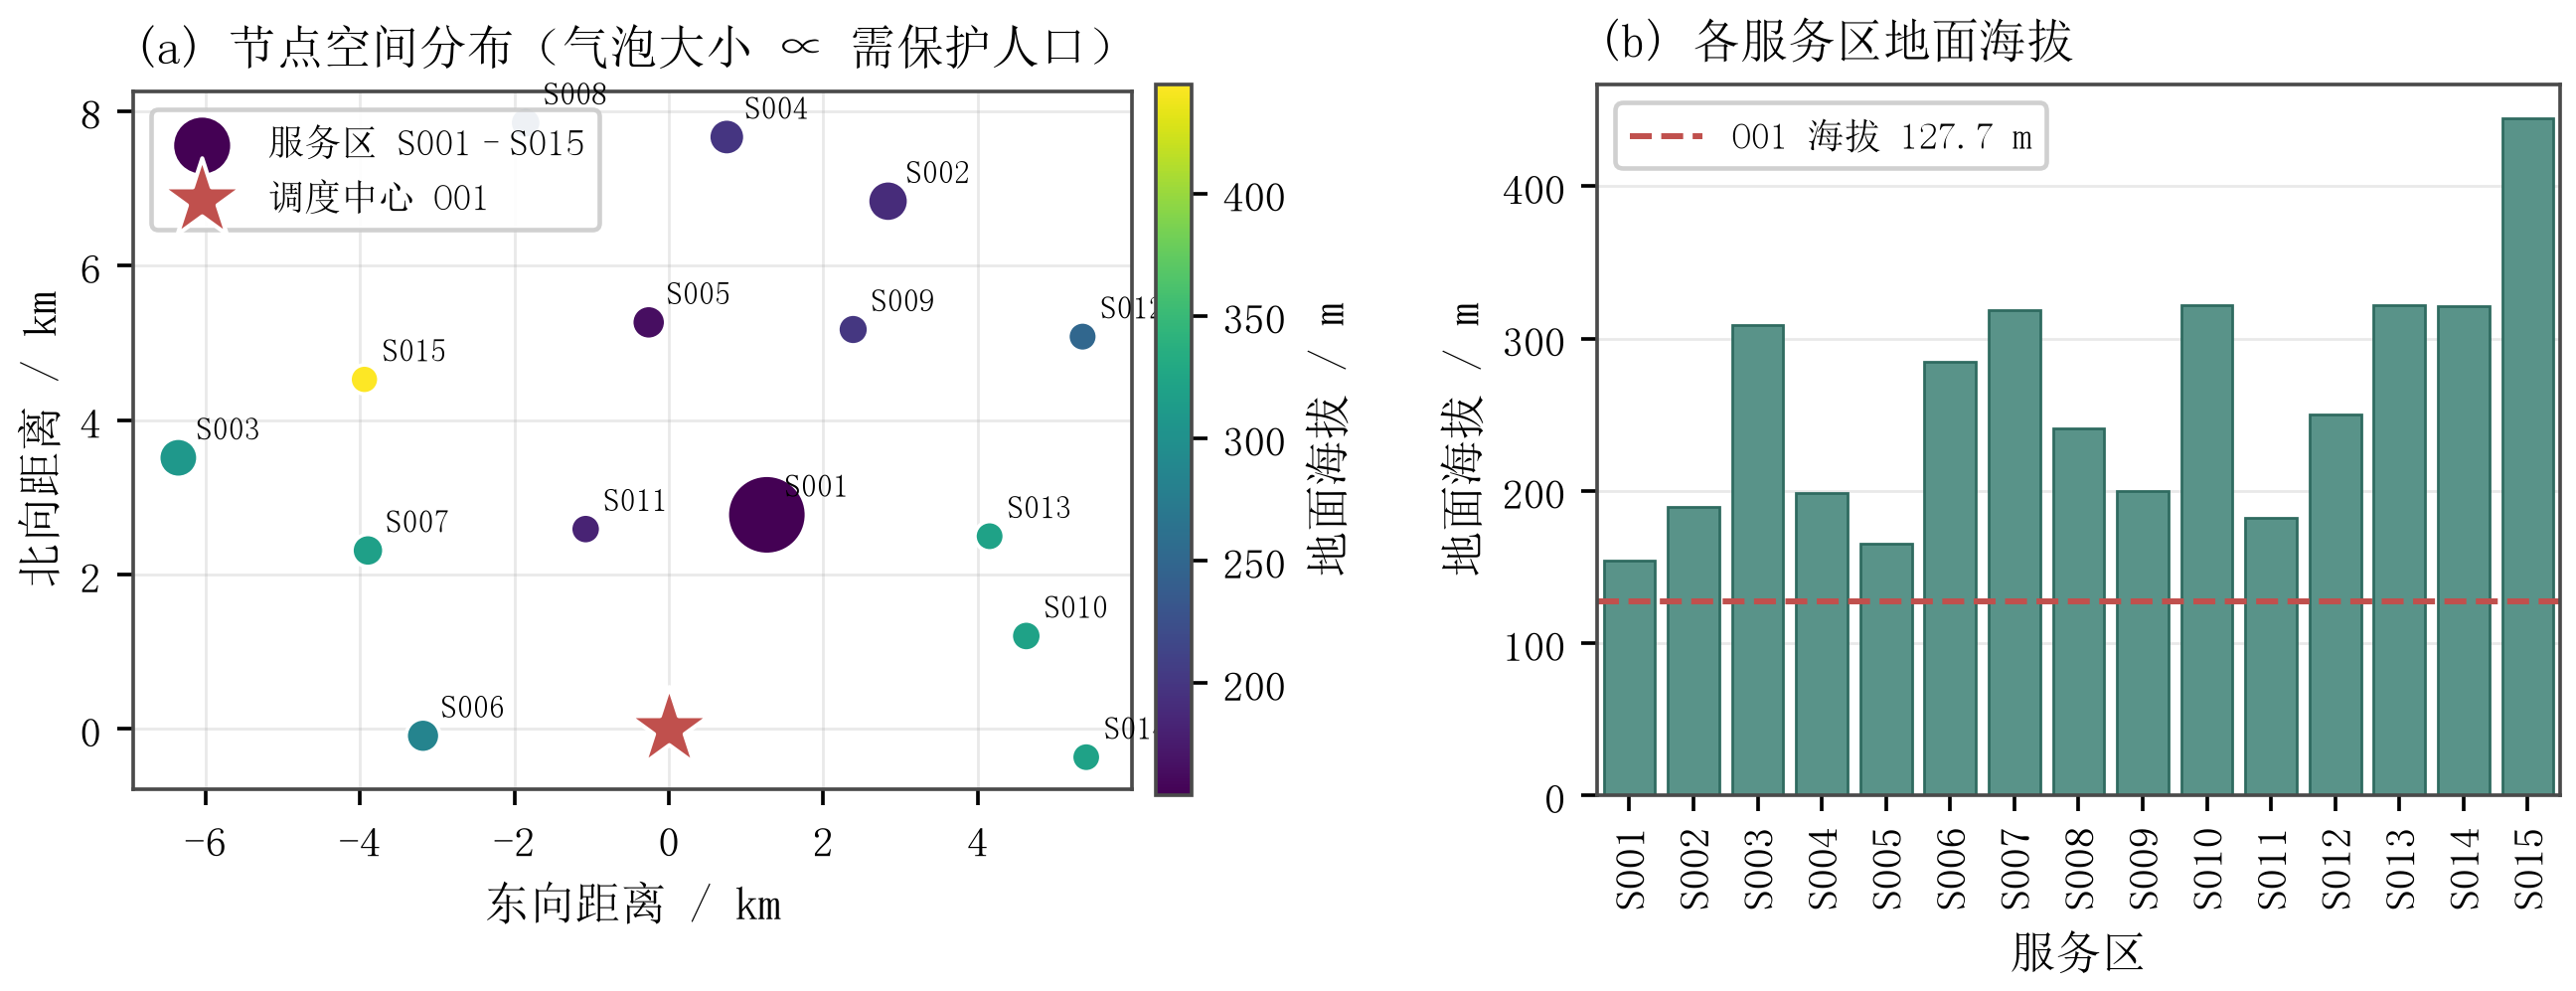
\includegraphics[width=0.98\textwidth]{figures/fig06_nodes.png}
	\caption{任务节点空间分布与地面海拔}
	\label{fig:nodes}
\end{figure}

如图~\ref{fig:nodes}(a) 所示，15 个服务区以调度中心 O01 为中心呈扇形分布，最远者（S008）距 O01 达 8.08\,km，最近者（S011）仅 2.81\,km；气泡大小反映需保护人口，S001 以 2100 人显著高于其他服务区。图~\ref{fig:nodes}(b) 显示服务区地面海拔差异悬殊，最低的 S001 为 154.0\,m，最高的 S015 达 444.5\,m，这一差异将通过爬升能耗直接影响各服务区的最大安全载荷。

需要强调的是，山区场景下航段的爬升高度并非由两端点海拔决定，而取决于\textbf{沿线最高地面高程}。图~\ref{fig:legs} 给出了全部 240 条有序航段的几何特征。

\begin{figure}[htbp]
	\centering
	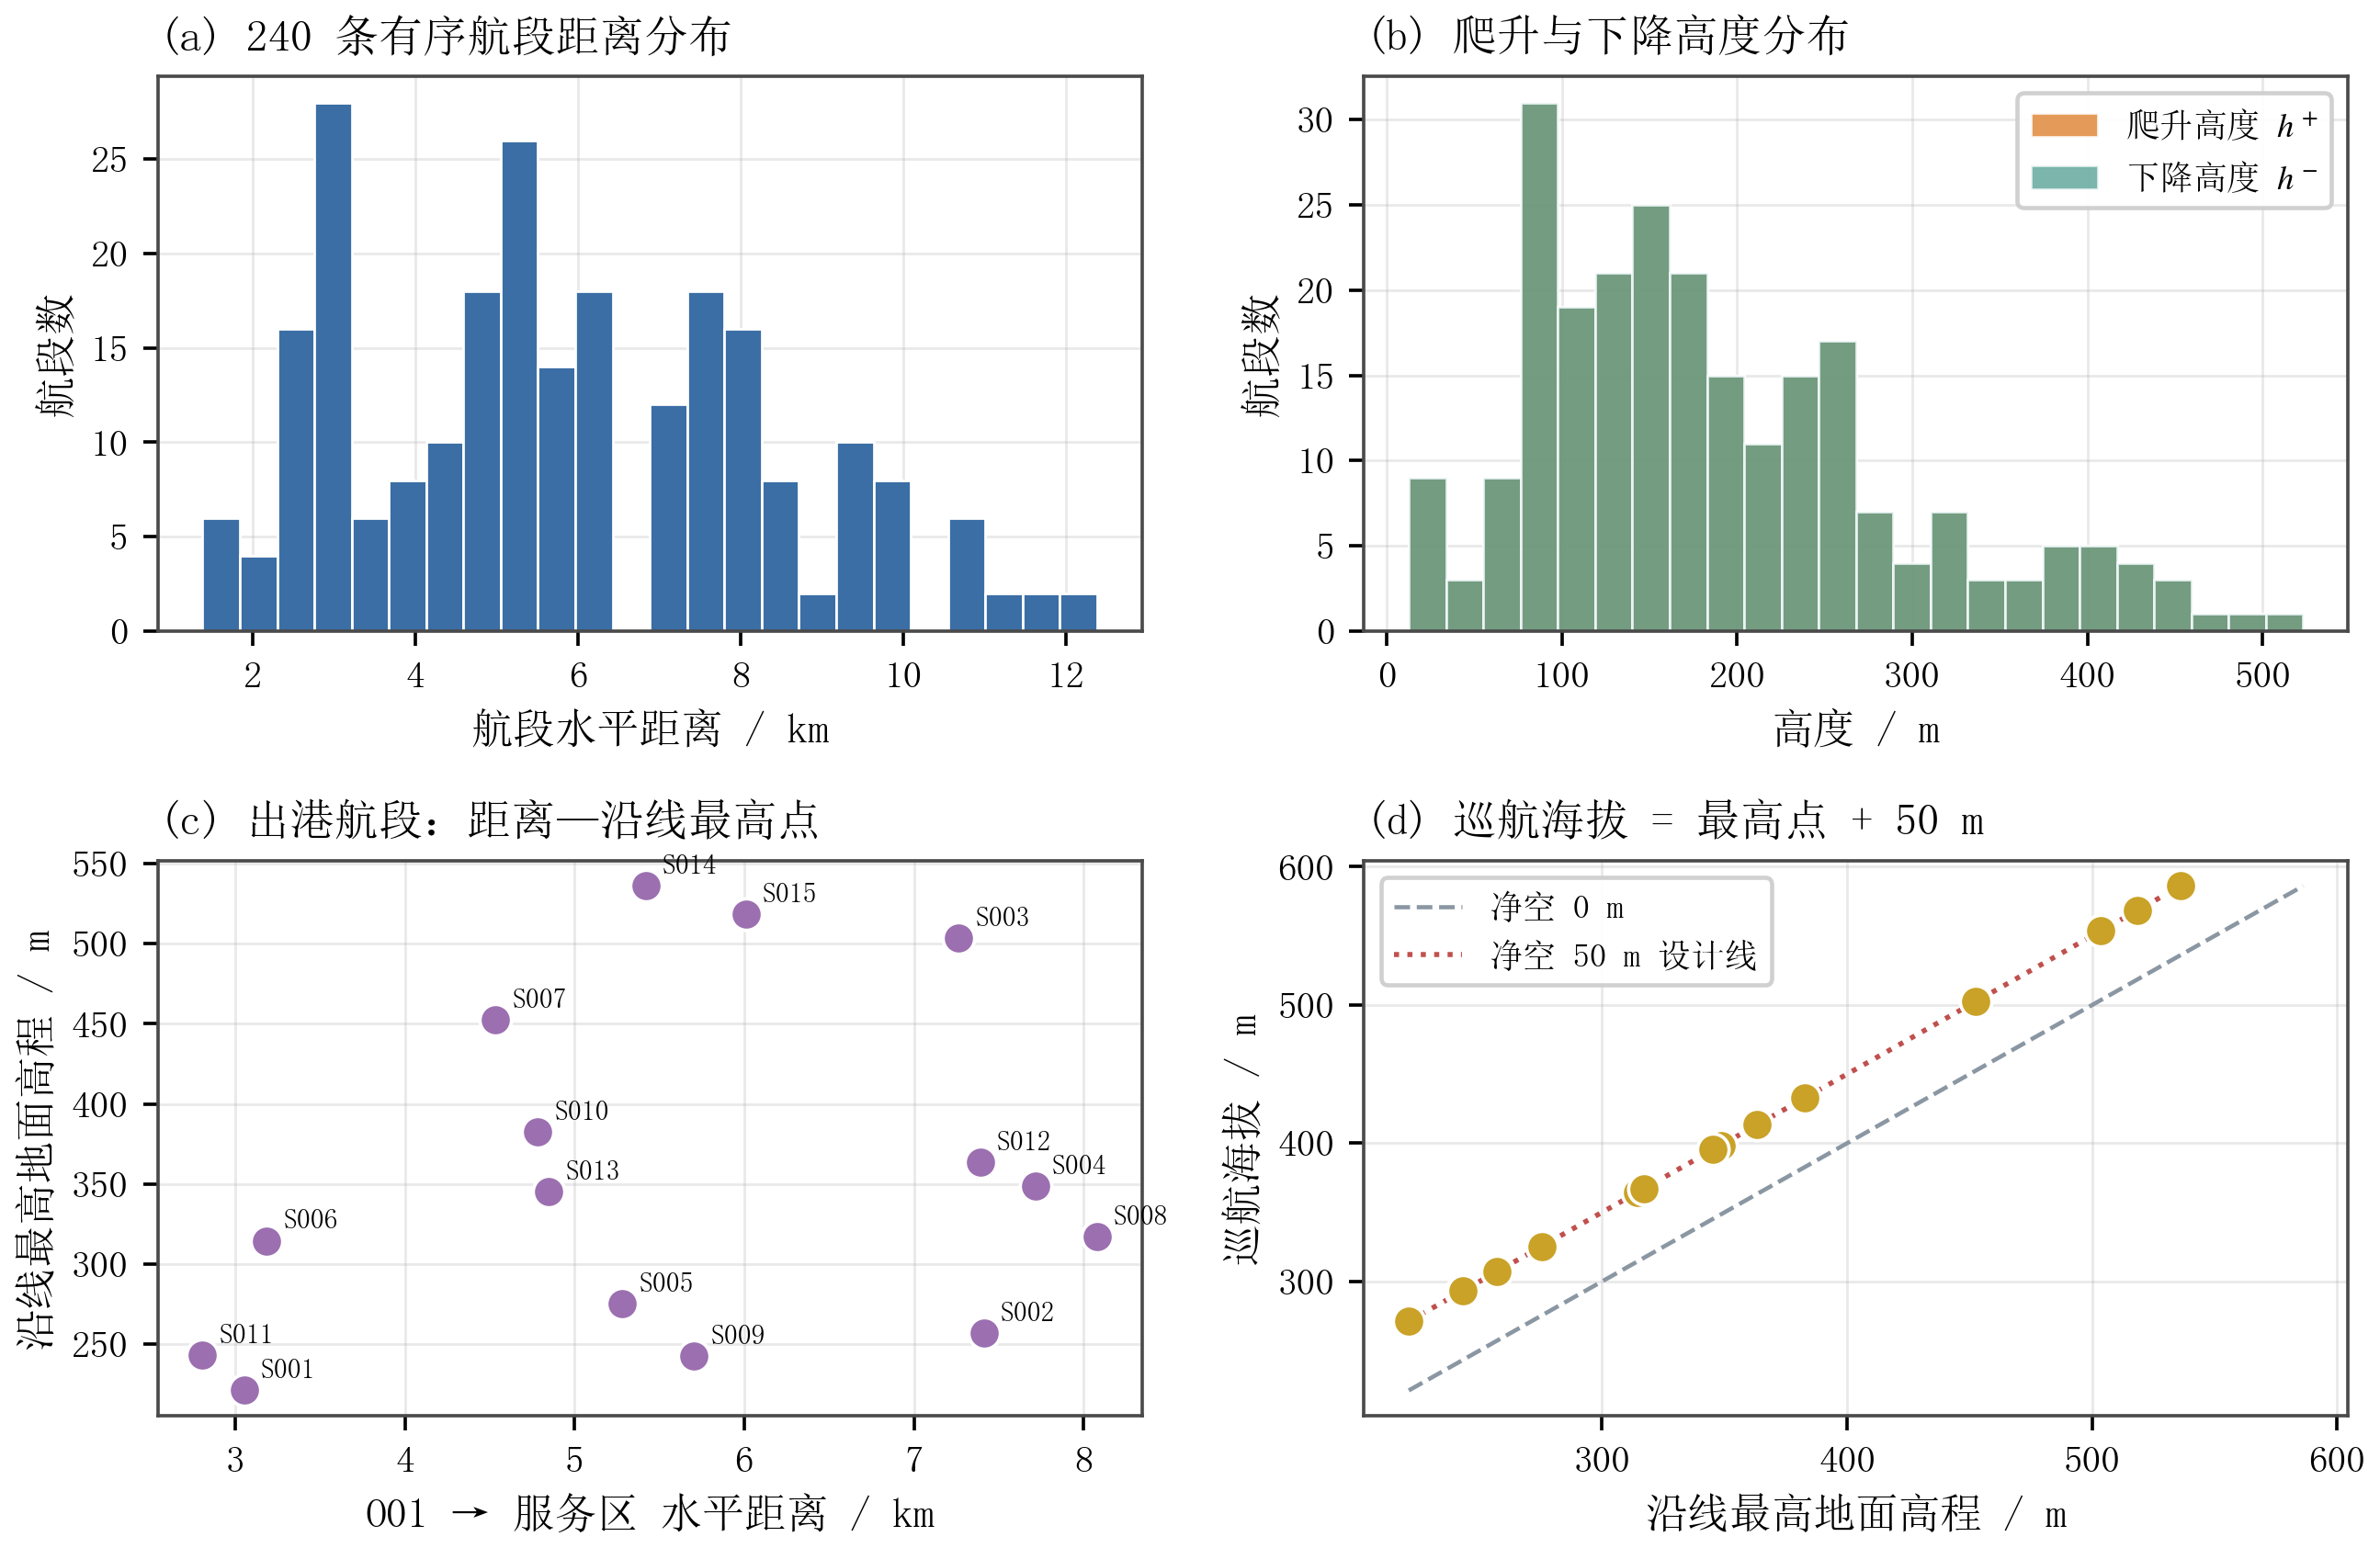
\includegraphics[width=0.98\textwidth]{figures/fig07_legs.png}
	\caption{航段几何特征与巡航海拔确定规则}
	\label{fig:legs}
\end{figure}

图~\ref{fig:legs}(a) 表明航段水平距离集中在 1.4$\sim$12.4\,km；图~\ref{fig:legs}(c) 显示各出港航段的沿线最高地面高程可达 536\,m，显著高于服务区自身海拔（如 S003 地面海拔 308.5\,m，但其航段沿线最高点为 503.6\,m），这印证了“必须沿航段采样最高点”这一口径的必要性——若只取两端点高程，将低估爬升高度约 200\,m，进而低估能耗。图~\ref{fig:legs}(d) 验证了本文采用的巡航海拔规则：所有航段均严格落在“最高点 $+50$\,m”的设计线上。

\subsubsection{物资与时限}

80 个货箱分为 4 类，其质量、体积与时限特征如表~\ref{tab:box_type} 与图~\ref{fig:boxes} 所示。

\begin{table}[htbp]
\caption{分类物资总量统计}
\label{tab:box_type}
\centering
\zihao{-5}
\setlength{\tabcolsep}{4pt}
\begin{tabular}{lccccc}
\toprule
物资类型 & 箱数 & 总质量/kg & 总体积/m$^3$ & 单箱质量/kg & 单箱体积/m$^3$ \\
\midrule
饮用水 & 36 & 504 & 0.972 & 14.0 & 0.027 \\
应急食品 & 19 & 152 & 0.532 & 8.0 & 0.028 \\
医疗物资 & 16 & 48 & 0.192 & 3.0 & 0.012 \\
生活卫生用品 & 9 & 54 & 0.315 & 6.0 & 0.035 \\
\textbf{合计} & \textbf{80} & \textbf{758} & \textbf{2.011} & — & — \\
\bottomrule
\end{tabular}
\end{table}


\begin{figure}[htbp]
	\centering
	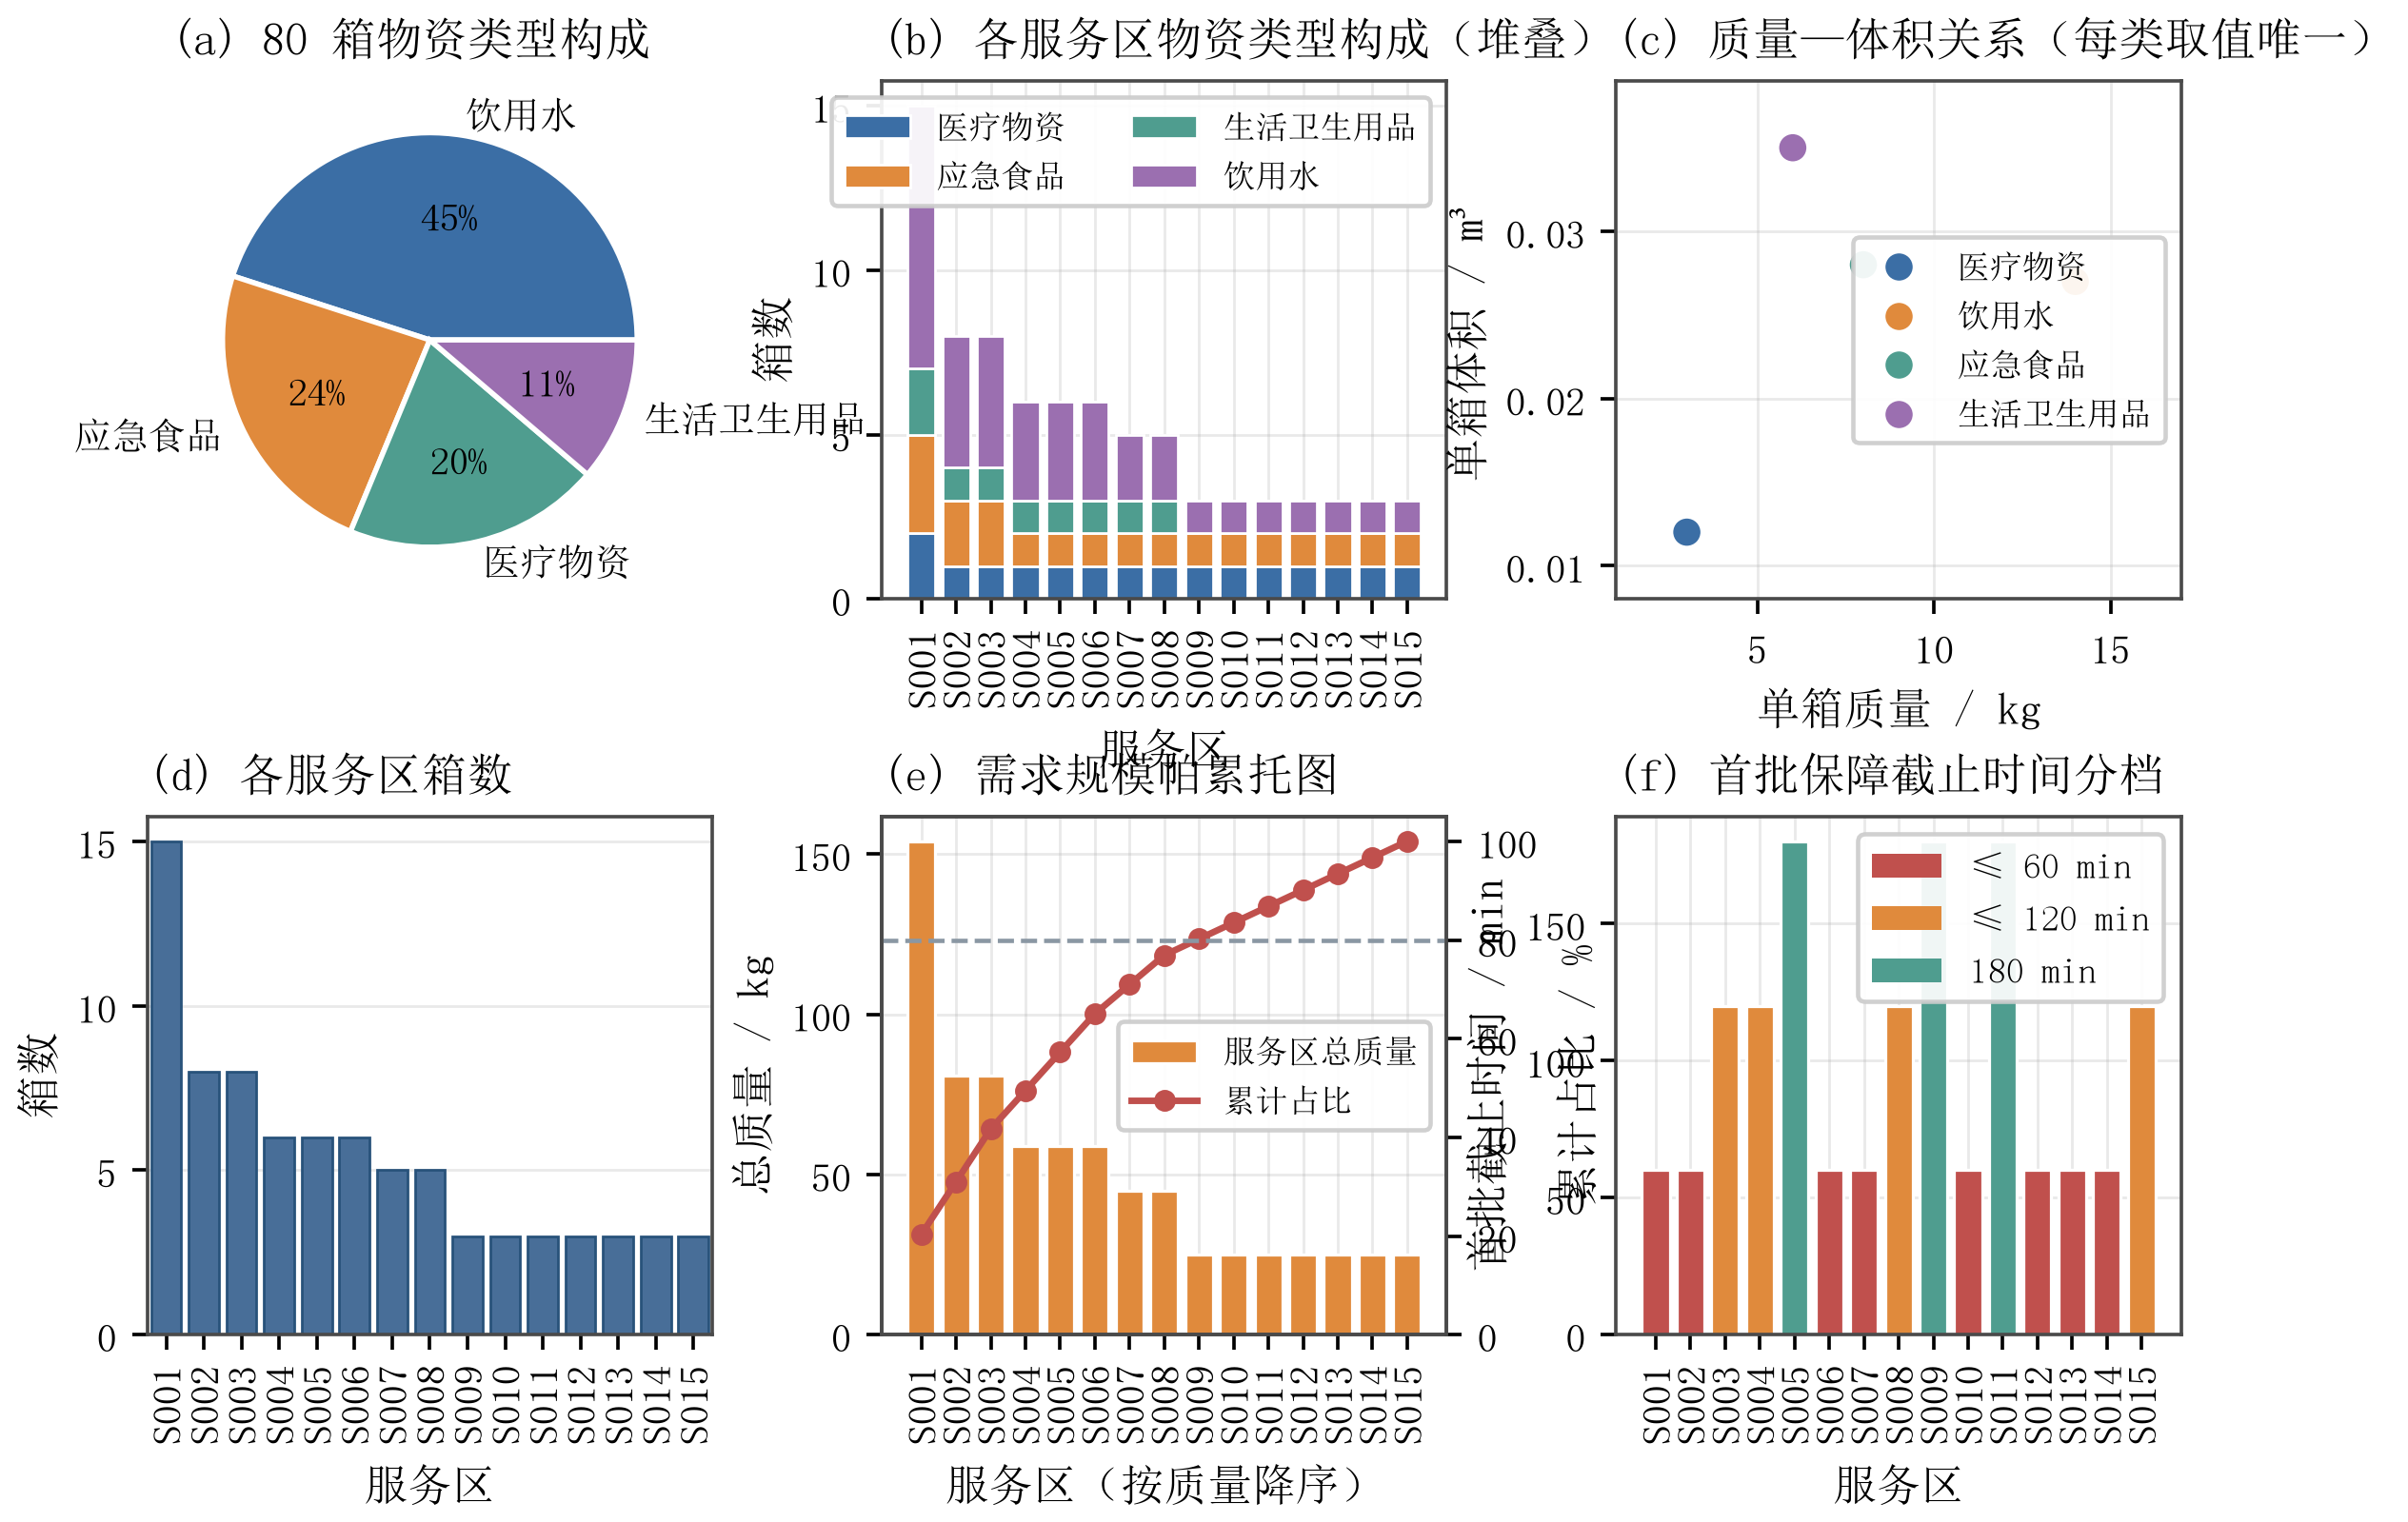
\includegraphics[width=0.98\textwidth]{figures/fig08_boxes.png}
	\caption{货箱数据特征}
	\label{fig:boxes}
\end{figure}

如图~\ref{fig:boxes}(a) 所示，饮用水箱数最多（36 箱，占 45\%），其次为应急食品（19 箱）、医疗物资（16 箱）与生活卫生用品（9 箱）。图~\ref{fig:boxes}(c) 揭示了一个对组批十分关键的事实：\textbf{同一类物资的单箱质量与体积取值唯一}（医疗 3\,kg/0.012\,$m^{3}$、饮用水 14\,kg/0.027\,$m^{3}$、应急食品 8\,kg/0.028\,$m^{3}$、生活卫生用品 6\,kg/0.035\,$m^{3}$），因此箱与箱之间不存在个体差异，组批问题退化为按类型计数的问题。值得注意的是\textbf{各类物资的“轻泡”程度差异很大}：生活卫生用品的单位质量体积为 5.83\,L/kg，而饮用水仅 1.93\,L/kg。这意味着\emph{质量约束与体积约束会在不同的服务区分别起主导作用}。

图~\ref{fig:boxes}(d) 显示 S001 的箱数（15 箱）远超其他服务区（多数为 3$\sim$8 箱），图~\ref{fig:boxes}(e) 的帕累托图进一步表明\textbf{前 4 个服务区（S001、S002、S003、S004）即占全部物资质量的约 47\%}，需求在空间上高度不均衡。

时限方面有两点必须严格区分：\textbf{首批截止时间}仅约束“是否首批保障 $=$ 是”的 30 个货箱，且每个服务区恰好 2 箱（医疗 1 $+$ 饮用水 1）；\textbf{期望送达时间}则对全部 80 箱都有约束。如图~\ref{fig:boxes}(f) 所示，首批截止时间呈 60/120/180\,min 三档分布，其中\textbf{8 个服务区的首批截止为 60\,min}（S001、S002、S006、S007、S010、S012、S013、S014）——这一数目恰好等于运输无人机总数（8 架），因此问题二只需让\textbf{每架无人机在 $t=0$ 各认领 1 个高紧迫服务区}，即可满足全部首批时限；反之，若把机队压缩为单一机型使用，这一“供给 $=$ 需求”的对偶就会被破坏（详见第~\ref{sec:q2} 节）。

\subsubsection{装备与链路}

3 种运输机型的核心参数如表~\ref{tab:uav_params} 所示。

\begin{table}[htbp]
\caption{三种运输机型主要参数}
\label{tab:uav_params}
\centering
\zihao{-5}
\setlength{\tabcolsep}{4pt}
\begin{tabular}{lccc}
\toprule
参数 & A 型 & B 型 & C 型 \\
\midrule
最大载货质量 $Q_{g}$ / kg & 25 & 30 & 80 \\
可用装载体积 $V_{g}$ / m$^3$ & 0.060 & 0.073 & 0.250 \\
巡航速度 $v_{g}^{c}$ / (m$\cdot$s$^{-1}$) & 12 & 15 & 15 \\
空载标准航程 $L_{g0}$ / km & 25 & 28 & 26 \\
满载标准航程 $L_{gF}$ / km & 20 & 16 & 12 \\
电池可用能量 $E_{g}^{use}$ / kWh & 4.5 & 4.0 & 8.0 \\
爬升速度 $v_{g}^{\uparrow}$ / (m$\cdot$s$^{-1}$) & 3.0 & 3.0 & 2.5 \\
下降速度 $v_{g}^{\downarrow}$ / (m$\cdot$s$^{-1}$) & 2.5 & 2.5 & 2.0 \\
基础交接时间 / s & 150 & 150 & 180 \\
每箱增加交接 / s & 30 & 30 & 36 \\
返航安全余量 $\rho_{g}$ & 20\% & 20\% & 20\% \\
共享电池组数 / 组 & 6 & 4 & 4 \\
等效完全充电时间 $T_{full}$ / s & 1800 & 2400 & 3000 \\
\bottomrule
\end{tabular}
\end{table}
三种机型的能力呈明显的“互补而非递进”关系：A 型航程最长（空载 25\,km）但载重最小（25\,kg）、货舱最小（0.06\,$m^{3}$）；C 型载重最大（80\,kg）、货舱最大（0.25\,$m^{3}$）但满载航程最短（12\,km），空载/满载航程衰减达 53.8\%。

\begin{figure}[htbp]
	\centering
	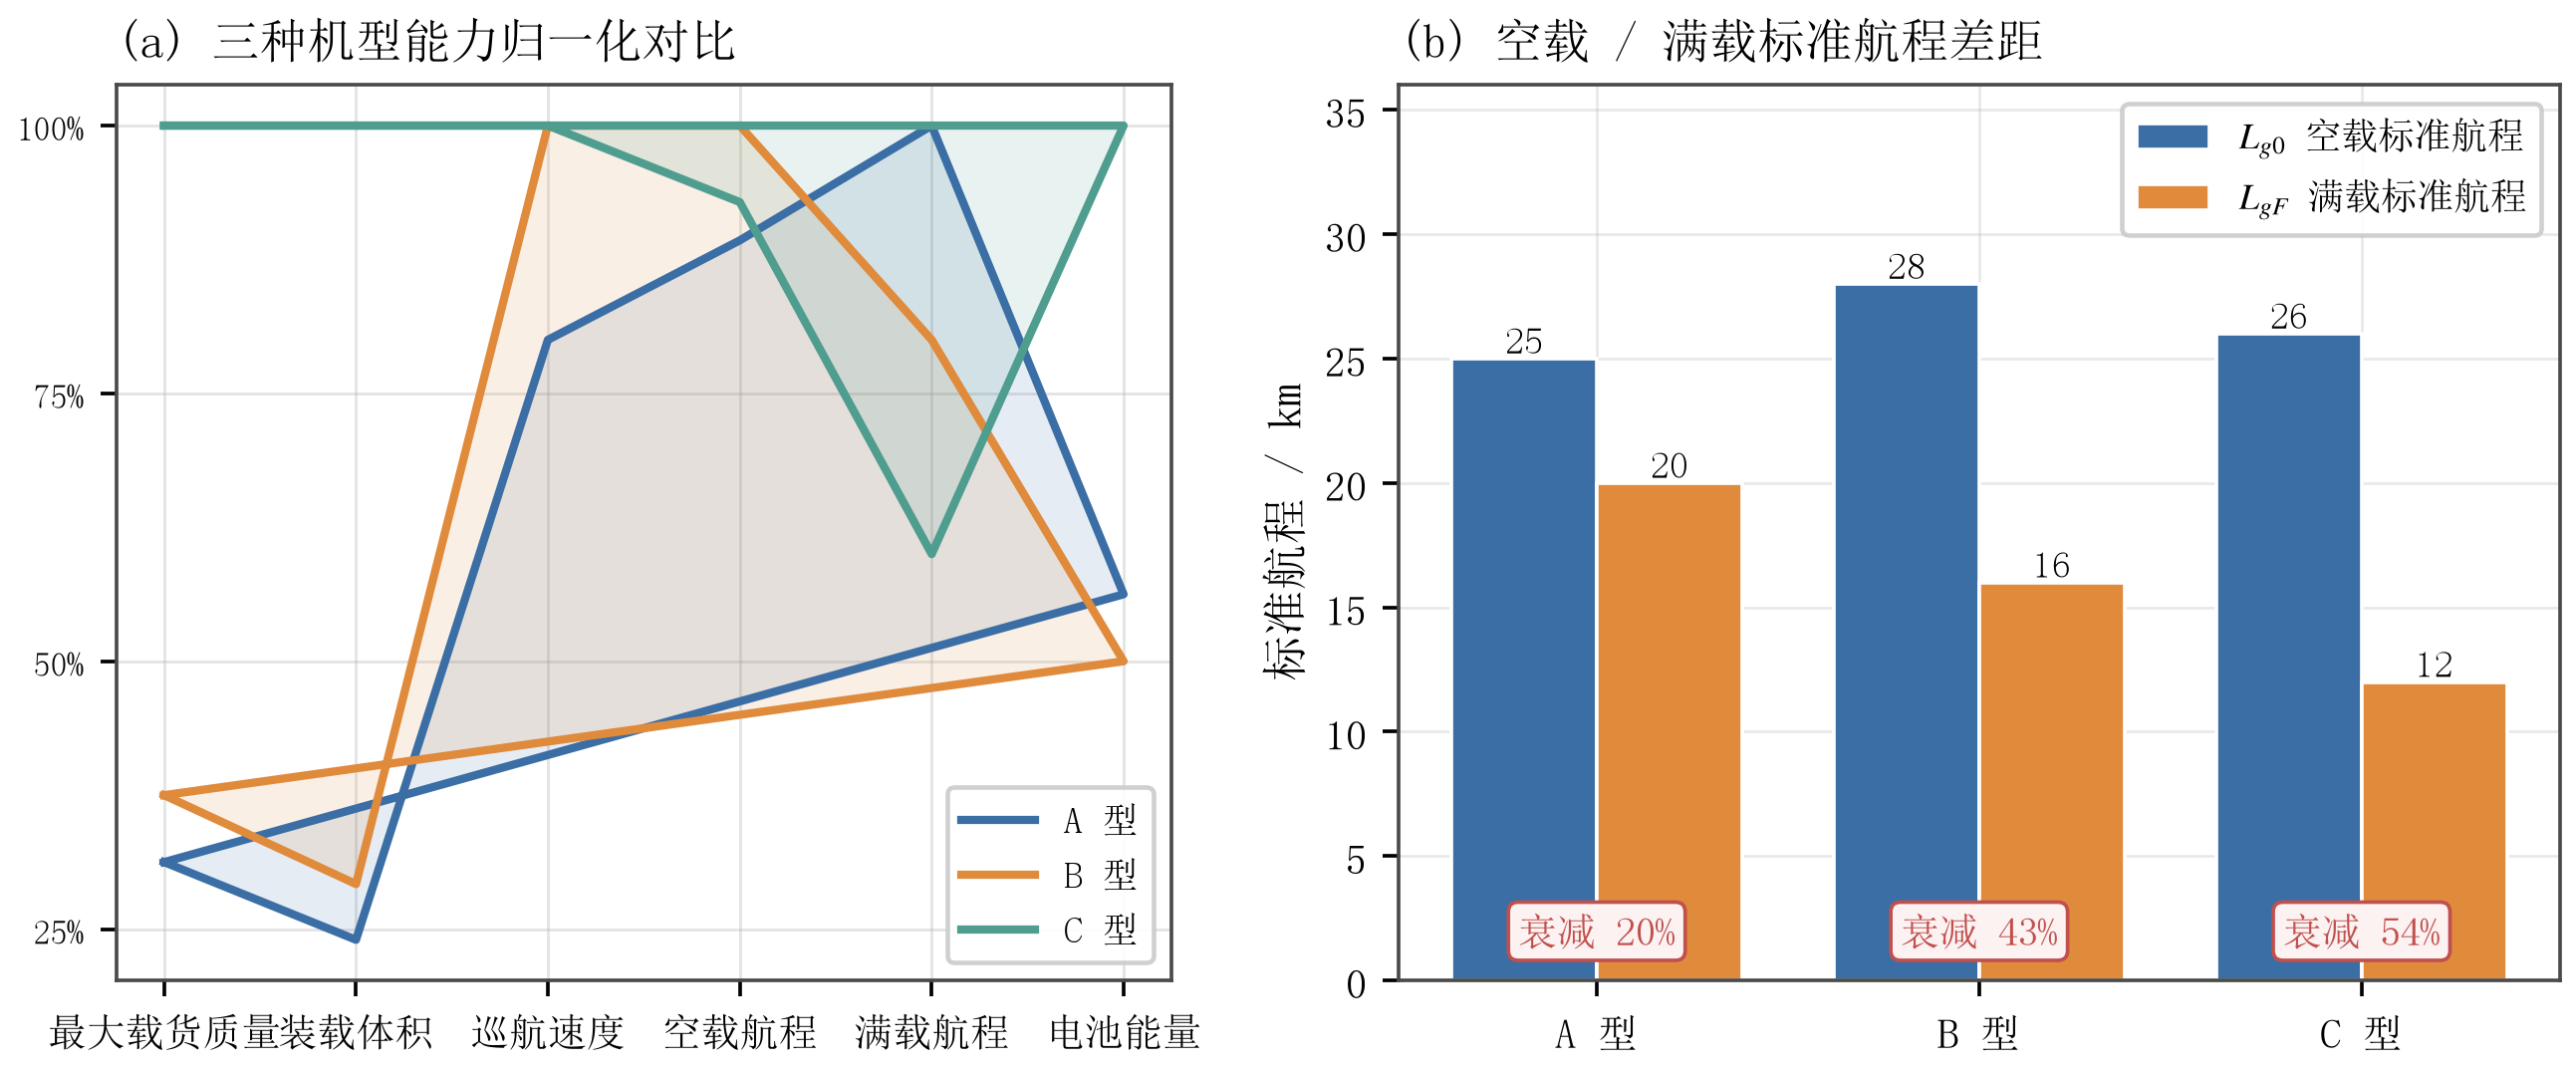
\includegraphics[width=0.98\textwidth]{figures/fig09_uav_radar.png}
	\caption{三种运输机型能力对比}
	\label{fig:uav_radar}
\end{figure}

图~\ref{fig:uav_radar}(a) 的归一化雷达图直观呈现了这一互补性：C 型在载货质量与装载体积两个维度上占优，A 型在航程维度上占优。图~\ref{fig:uav_radar}(b) 强调了一个容易被忽视的事实——\textbf{满载航程相对空载航程的衰减幅度差异极大}：A 型仅衰减 20\%，而 C 型高达 53.8\%。正是这一差异，使得重载机型在远距离任务中会率先触及能量约束。

通信链路参数方面\cite{zeng2016uavcomm}，附件对固定网关 G01、运输无人机、中继接入端与中继回传端分别给出了发射功率与天线增益。需要特别注意的是，附件\textbf{用单一符号 $G$ 表示天线增益}，即题目公式中的 $G_t$ 与 $G_r$ 取同一数值，但各主体取自身参数值。据此计算的链路预算如表~\ref{tab:link_thresholds} 与图~\ref{fig:link} 所示。

\begin{figure}[htbp]
	\centering
	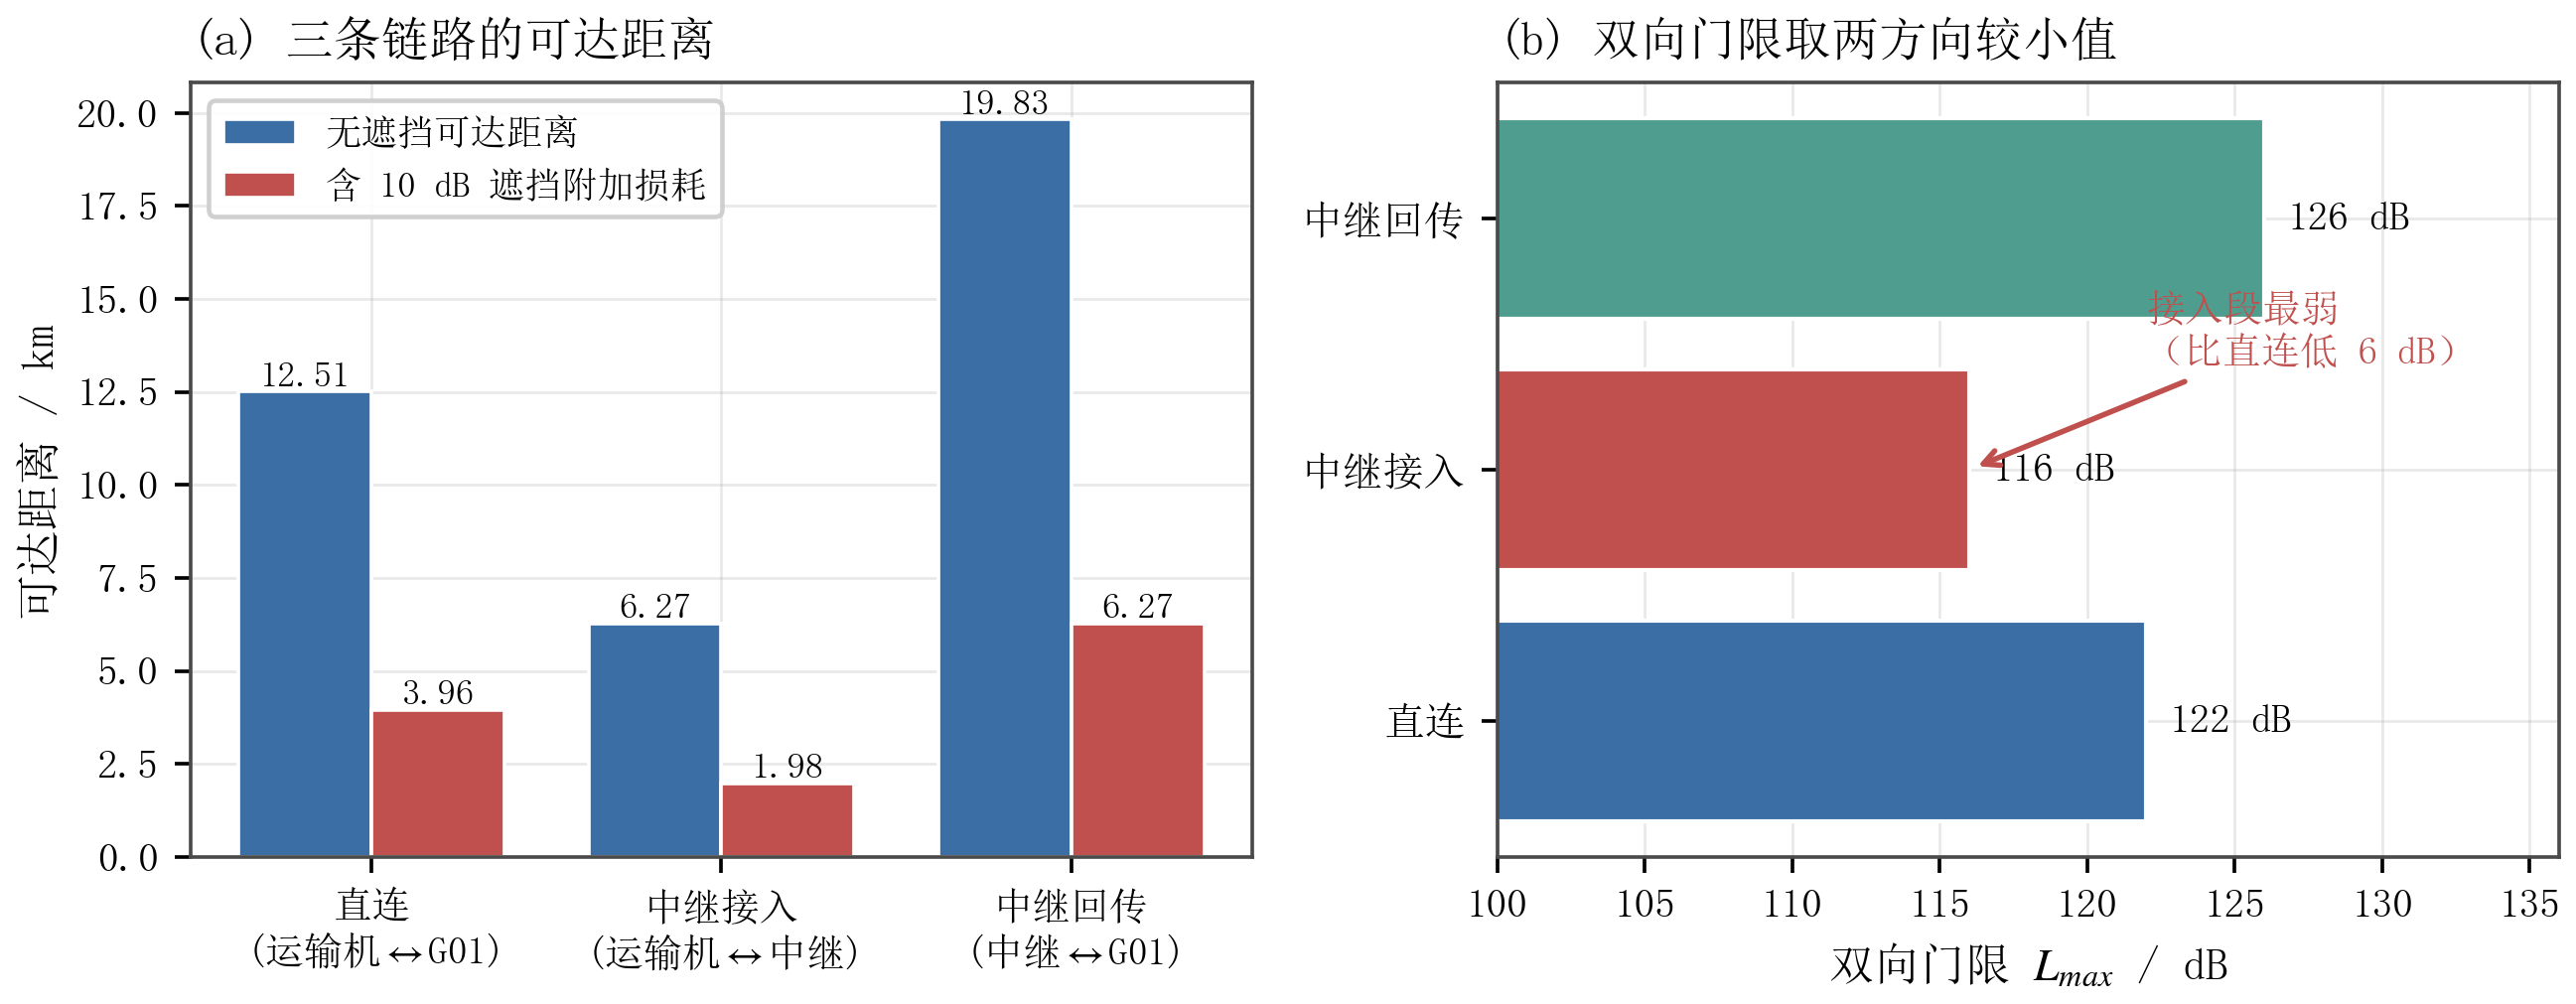
\includegraphics[width=0.98\textwidth]{figures/fig10_link.png}
	\caption{通信链路预算与双向门限}
	\label{fig:link}
\end{figure}

由图~\ref{fig:link}(b) 可见，三条链路的双向门限依次为\textbf{直连 122\,dB、中继接入 116\,dB、中继回传 126\,dB}。中继接入段（运输机 $\leftrightarrow$ 中继）的门限\textbf{比直连还低 6\,dB}，这是“中继并不总是更好”的量化依据。图~\ref{fig:link}(a) 进一步给出可达距离：接入段在无遮挡时仅 6.27\,km，叠加 10\,dB 地形遮挡附加损耗后骤降至 1.98\,km。这两条结论共同决定了问题三中继选址的基本形态——\textbf{中继必须贴近运输无人机作业空域，而非贴近网关}。
